\documentclass[10pt,a4paper]{article}
\usepackage[utf8]{inputenc}
\usepackage{graphicx}
\usepackage{amsmath}
\usepackage{hyperref, cite}
\usepackage[top=2.5cm, bottom=2.5cm, left=2.5cm, right=2.5cm]{geometry}
\usepackage{titling}
\usepackage{subfig}
\usepackage{enumitem}
\usepackage{float}

\title{Distributed Video Detection Using YOLO, Kafka and Spark \\[0.5cm] 
\large CSIT5970 Course Project -- Group 8}
\author{
    JIANG Yihang \\ 
    LIU Yishan \\
    ZHAO Tianci
}

\begin{document}
\maketitle

\section{Background}
The proliferation of video data in modern applications ranging from surveillance systems to live streaming platforms has created an urgent need for efficient real-time analysis solutions. Traditional video processing systems often struggle with scalability and latency when handling high-resolution footage, particularly when deploying compute-intensive deep learning models like YOLO (You Only Look Once) for object detection. This project addresses these challenges by leveraging distributed computing paradigms, combining Kafka's high-throughput messaging capabilities with Spark's stream processing engine to enable horizontal scaling across cloud infrastructure. The resulting system provides a blueprint for implementing cost-effective, production-grade video analytics pipelines that can adapt to fluctuating workloads while maintaining sub-second detection latency.

\section{Introduction}
\subsection{Project Architecture}
Our distributed YOLO video detection system adopts a cloud-native microservices architecture built on Kubernetes orchestration, as illustrated in Figure~\ref{fig:arch}. This design separates concerns through four functional layers: client interaction, distributed streaming, AI processing, and persistent storage. This architecture enables horizontal scaling to handle high-resolution video streams at reasonable performance.

\begin{figure}[htbp]
    \centering
    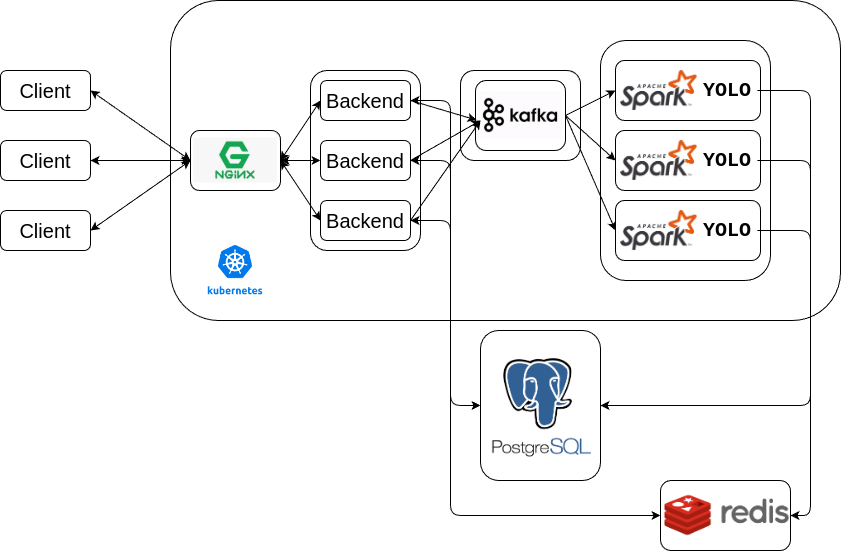
\includegraphics[width=0.85\textwidth]{arch.png}
    \caption{System Architecture Diagram}
    \label{fig:arch}
\end{figure}

\subsection{Core Components \& Responsibilities}
\begin{itemize}
    \item \textbf{Client Interface}: Handles video upload via HTTP/HTTPS and polling-based result fetching
    \item \textbf{Nginx Ingress}: Routes external traffic to backend services
    \item \textbf{Backend Server}: Performs frame extraction, processing status query and result construction
    \item \textbf{Kafka Cluster}: Acts as a distributed message buffer for video frames
    \item \textbf{Spark Streaming}: Executes YOLO inference with potential GPU node acceleration
    \item \textbf{Database Layer}: PostgreSQL for persist result storing \& Redis for temporary result caching
    \item \textbf{Kubernetes Orchestration}: Hosts backend, Kafka and Spark as scalable pods
\end{itemize}

\subsection{Video Processing Workflow}
The distributed video analysis pipeline operates through four coordinated phases, as depicted in Figure~\ref{fig:workflow}:

\begin{figure}[htbp]
    \centering
    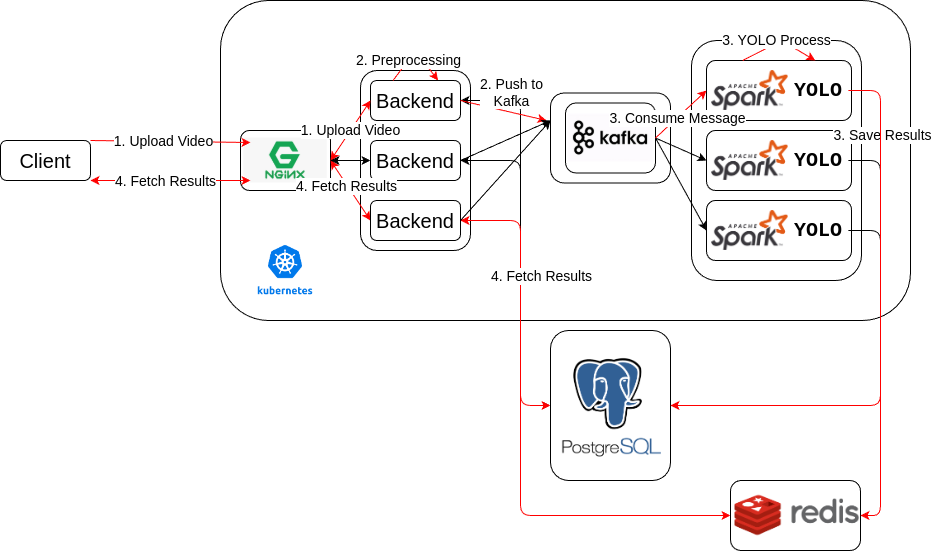
\includegraphics[width=0.9\textwidth]{workflow.png}
    \caption{Video Processing Workflow}
    \label{fig:workflow}
\end{figure}

\begin{enumerate}
    \item \textbf{Upload Phase}: Client upload the target video to backend service through load-balanced Nginx Ingress
    \item \textbf{Preprocessing Stage}: Backend extracts video frames and publishes to Kafka topic
    \item \textbf{Stream Processing}: Spark workers get the video frames from Kafka topic and process the frames using YOLO, saving the results to PostgreSQL and update Redis cache
    \item \textbf{Result Fetching}: Client periodically query the backend service for processing status, and gets the results when the processing is completed
\end{enumerate}

\section{Implementation Details}
\subsection{Client}

\subsubsection{Video Upload Workflow}
The file upload process follows a robust validation and chunked transfer mechanism as illustrated in Figure~\ref{fig:client-wf-upload}. The workflow begins with CLI argument parsing and input path verification using \texttt{os.path.getsize} for file existence checks. For valid files, the implementation calculates exact byte size to initialize a \texttt{tqdm} \cite{tqdm_docs} progress bar. The chunked upload mechanism employs a custom \texttt{UploadProgressWrapper} class to stream video content through \texttt{requests.post} with HTTP \cite{python_requests_upload}. Successful responses (HTTP 200) return the server-generated \texttt{job\_id}, while error states trigger specific exception handling for network failures and invalid JSON responses.

\begin{figure}[htbp]
    \centering
    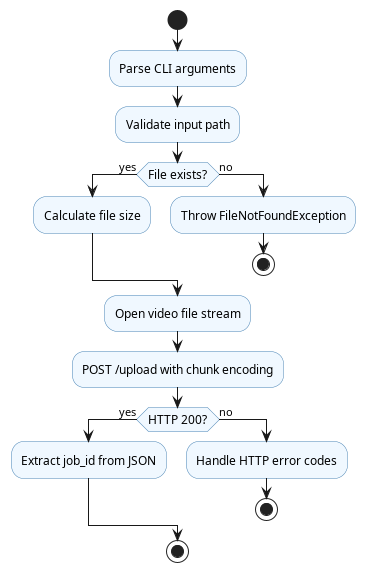
\includegraphics[height=10cm]{client-wf-upload.png}
    \caption{Video Upload Workflow}
    \label{fig:client-wf-upload}
\end{figure}

\subsubsection{Job Polling Workflow}
Figure~\ref{fig:client-wf-polling} demonstrates the state-aware polling mechanism with backoff retry logic. The implementation initializes a retry counter and enters a persistent polling loop using \texttt{requests.get} \cite{python_requests_upload} to query the \texttt{/job/\{job\_id\}} polling API endpoint. The state machine handles four response conditions:
\begin{itemize}
    \item \textbf{Success (0)}: Closes progress bars and returns results
    \item \textbf{Processing (1)}: Updates frame-level progress using \texttt{processed\_frames} counter
    \item \textbf{Failed (2)}: Immediately raises execution exceptions
    \item \textbf{Network Errors}: Implements 5-second delayed retries with counter-based max retry times limit
\end{itemize}

\begin{figure}[htbp]
    \centering
    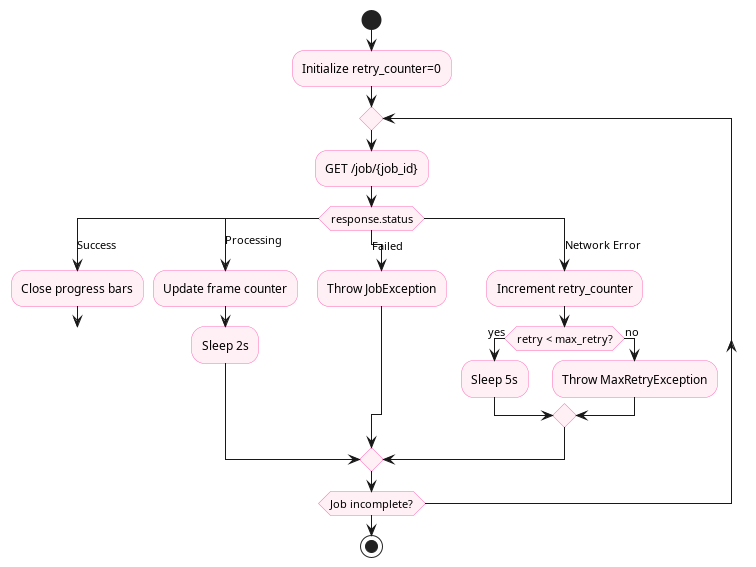
\includegraphics[height=10cm]{client-wf-polling.png}
    \caption{Job Polling Workflow}
    \label{fig:client-wf-polling}
\end{figure}

\subsubsection{Result Processing Workflow}
The frame processing pipeline shown in Figure~\ref{fig:client-wf-render} combines computer vision operations with result processing. Using \texttt{cv2.VideoWriter} with MP4V encoding \cite{opencv_docs}, the implementation:
\begin{enumerate}
    \item Generates HSV-based color maps using golden ratio distribution for class differentiation
    \item Processes frames sequentially with confidence threshold filtering (\texttt{confidence\_threshold} parameter)
    \item Renders bounding boxes and text labels using OpenCV's vector drawing functions
    \item Outputs frame-by-frame detection results in JSON format
\end{enumerate}
The dual output files (annotated video + JSON) ensures result reproducibility.

\begin{figure}[htbp]
    \centering
    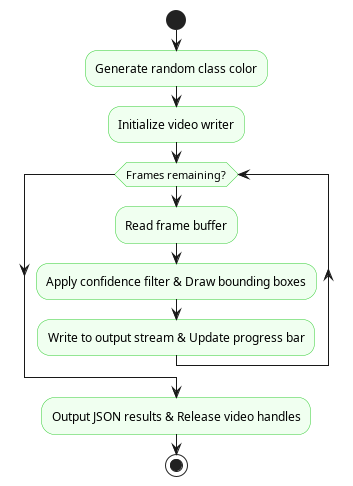
\includegraphics[height=9cm]{client-wf-render.png}
    \caption{Result Process Workflow}
    \label{fig:client-wf-render}
\end{figure}

\subsubsection{Dockerization Strategy}

A Docker image is created for the client following cloud-native best practices \cite{docker_best_practices}. Utilizing the \texttt{python:3.12-slim-bookworm} base image minimizes image size while maintaining Python compatibility. The Docker image supports flexible deployment scenarios with volume mounting for persistent storage for input/output videos and command line argument passing.

\subsection{Backend}

TODO: add backend section

\subsection{Spark Job: YOLO Detection}

TODO: add spark job section

\section{Deployment}
\subsection{Nginx Ingress Controller}
Our deployment leverages Nginx Ingress Controller \cite{nginx_ingress} as the Kubernetes-native traffic orchestration layer, providing essential capabilities for managing external access to the video processing backend service. The implementation combines cloud-native design principles with performance optimizations for heavy video payloads. Our Nginx Ingress controller contains several critical configurations:

\begin{itemize}
    \item \texttt{rewrite-target} annotation ensures proper URI mapping between external routes and internal service endpoints, crucial for maintaining API consistency across distributed components

    \item \texttt{proxy-body-size} adjustment to 2GB accommodates large video frame batches in Base64 encoding format, exceeding the default 1MB limit

    \item Host-based routing isolates requests for different services
\end{itemize}

\subsection{Backend}
The backend service employs Kubernetes Horizontal Pod Autoscaler (HPA) \cite{kubernetes_hpa} to maintain responsive video ingestion during workload spikes while optimizing resource utilization. The HPA configuration scales the backend deployment between 2-N replicas based on CPU utilization (50\% target). This design ensures efficient handling of video upload bursts through pod cloning while preventing over-provisioning during idle periods.

\subsection{Kafka}
The Kafka deployment leverages Strimzi Operator \cite{strimzi} for Kubernetes-native Kafka cluster management, enabling declarative configuration and automated scaling. Strimzi simplifies deployment through custom resource definitions (CRDs) like \texttt{Kafka} and \texttt{KafkaNodePool}, which manage broker lifecycle, persistent storage, and KRaft mode coordination. The Strimzi solution supports seamless transition from development to production through configuration inheritance and environment-specific overrides.

\subsection{Spark}
Our Spark job deployment leverages \texttt{spark-operator} \cite{spark_operator} to achieve Kubernetes-native lifecycle management and elastic scaling of distributed video processing tasks. Our configuration demonstrates three key architectural advantages:

\begin{itemize}
    \item \textbf{Declarative Job Management}: SparkApplication CRD (Custom Resource Definition) enables version-controlled job specifications with embedded Kafka connection parameters, eliminating manual \texttt{spark-submit} operation
    \item \textbf{Resource Granularity}: Per-executor pod resource definitions (memory,cpu etc.) allow fine-grained resource allocation
    \item \textbf{Horizontal Scaling}: The operator's controller watches Kubernetes API for resource availability, dynamically adjusting executor counts through \texttt{spec.executor.instances} updates during workload spikes
\end{itemize}

\subsection{Database}
The database layer adopts an externalized architecture with standalone PostgreSQL and Redis instances outside the Kubernetes cluster, prioritizing three key operational advantages:

\begin{itemize}
    \item \textbf{Performance Gain}: Avoids performance overhead (network-attached volumes, pod scheduling latency) for consistent sub-millisecond response times
    \item \textbf{Data Durability}: Enables filesystem-level snapshots and physical backup strategies
    \item \textbf{Operational Simplicity}: Bypasses statefulset complexities for in-cluster deployment
\end{itemize}

\section{Conclusion}

TODO: add highlights, possible improvements etc...

\begin{thebibliography}{9}
    \bibitem{tqdm_docs} tqdm Progress Bars Documentation, https://tqdm.github.io
    \bibitem{python_requests_upload} Python Requests Library Documentation, https://docs.python-requests.org
    \bibitem{opencv_docs} OpenCV Video Processing Guide, https://docs.opencv.org
    \bibitem{docker_best_practices} Docker Python Best Practices, https://docs.docker.com/language/python
    \bibitem{nginx_ingress} Nginx Ingress Controller, https://github.com/kubernetes/ingress-nginx
    \bibitem{kubernetes_hpa} Kubernetes Horizontal Pod Autoscale, https://kubernetes.io/docs/tasks/run-application/horizontal-pod-autoscale
    \bibitem{strimzi} Strimzi Operator for Kafka, https://strimzi.io/documentation
    \bibitem{spark_operator} Spark Operator, https://github.com/kubeflow/spark-operator
\end{thebibliography}

\end{document}